\documentclass[14pt,a4paper,russian]{article}
% \documentclass[14pt,a4paper]{extarticle}
\usepackage[14pt]{extsizes}
\usepackage[utf8]{inputenc} 
\usepackage[T2A]{fontenc} % before babel!
\usepackage[english, russian]{babel}
\usepackage[titletoc]{appendix}
\usepackage{amsmath}
\usepackage{amssymb}
\usepackage{bm}
\usepackage{babel,blindtext}  
\usepackage[backend=bibtex,style=numeric]{biblatex}  %backend=biber is 'better'  


%\usepackage{polyglossia}


\usepackage{caption}
\usepackage{color}
\usepackage{epigraph}
\usepackage{epsfig}
\usepackage{enumitem}
\usepackage{float}
\usepackage{textcomp}
\usepackage{gensymb}
\usepackage{graphicx}
\usepackage{hyperref}   
\usepackage{mathtools}
\usepackage{lipsum}
\usepackage{indentfirst,latexsym}
\usepackage{physics}
\usepackage{setspace}
\usepackage{subcaption}

\graphicspath{{img/}}

\addbibresource{kursach.bib}
%\selectlanguage{russian}

\onehalfspacing

%\usepackage{fontspec}
%\usepackage{polyglossia}
%\setmainfont[Ligatures=TeX]{cmunrm.otf}
%% \setmainfont[Ligatures=NoCommon]{Times New Roman}
%\setmainlanguage{russian}
%\setotherlanguage{english}
%\newfontfamily\cyrillicfonttt{lmmonolt10-bold.otf}


%% \newcommand{\be}{\begin{equation}}
%% \newcommand{\ee}{\end{equation}}
%% newcommand{\df} {\mathop{}\!\mathrm{d}}


\textheight 25.7cm % 29.7-2-2=25.7
\textwidth 17cm % 21-2.5-1.5=17.0
\hoffset -0.04cm %2.5-2.54=-0.04 слева 3см
\voffset -1.04cm %2-2.54=0.54 сверху 2см
\oddsidemargin 0cm
\headheight 0cm
\headsep 0cm
\topmargin 0cm
\setcounter{page}{1}
\def\sigspace{\\[1em]
\underline{\hspace{5cm}}\\[-0.2em]}




\begin{document}

\begin{titlepage}
	\begin{center}
		{
		{\bf Санкт-Петербургский Государственный Университет\\
		\vskip 1em
		Математико-механический факультет\\
		Кафедра Астрономии} }

	\vspace{3cm}
    	
	{\large А.С.\,Патшин}
    
    \vskip 2em
    

	\Large{\bf{Сравнение тригонометрических параллаксов звезд TGAS и Hipparcos}}
    \vskip 1em
    {\normalsize {Дипломная работа}\\}
	\end{center}
	
	\vskip 5em
    
	{
		 \begin{flushright}
			Научный руководитель:\\
		    доцент А.С.\,Цветков\sigspace
		    Рецензент:\\
		    PhD. З.М.\,Малкин\sigspace
		\end {flushright}
	}

	\vfill
	\begin{center}
	\small {Санкт-Петербург

	2018}
	\end{center}
\end{titlepage}

\newpage
\begin{titlepage}
	\begin{center}
		{
		{\bf Saint-Petersburg State University\\
		\vskip 1em
		Mathematics and Mechanics Department\\
		Chair of Astronomy} }

	\vspace{3cm}
    	
	{\large Anton Patshin}
    
    \vskip 2em
    

	\Large{\bf{Comparison of trigonometric parallaxes of TGAS and Hipparcos stars}}
    \vskip 1em

    {\normalsize {Graduation Thesis}\\}
	\end{center}
	
	\vskip 5em
    
	{
		 \begin{flushright}
			Scientific supervisor:\\
		    associate professor Alexander Tsvetkov\sigspace
		    Reviewer:\\
		    PhD. Zinovy Malkin \sigspace
		    
		\end {flushright}
	}

	\vfill
	\begin{center}
	\small {Saint-Petersburg

	2018}
	\end{center}
\end{titlepage}
\newpage
\tableofcontents
\newpage



 
\section{Введение}\label{introduction}

(Переписать этот пример под мою работу)


Сравнение каталогов является класической задачей фундаментальной\\ астрометрии, производщей переход от отдной системы координат к другой, оценить уровень систематических ошибок. До недавненго времени могло проводиться сравнение лишь положений и собственных движений.Появление первых результатов миссии GAIA, в частности, каталога TGAS, позволило впервые проихвести сравение тригонометрических параллаксов общих звезд каталогов TGAS и  Hipparcos, а именно его второй версии XHIP (XHIP: An extended hipparcos compilation, Anderson, 2012). Каталог TGAS содержит 2057050 звезд с данными о тригонометрических параллаксах, включает в себя только звезды Hipparcos и Tycho-2  и не является в полном смысле независимым продуктом, т.к. использует в качестве первой эпохи данные этих двух каталогов. Для сравнения мы используем общие звезды XHIP  и TGAS, которых оказалось 93635, из которыз пригодно для анализа 90282.

\subsection{Общие сведенья о GAIA и TGAS}\label{sub:smthgaia}
Каталог GAIA
		
\subsection{Общие сведенья о Hipparcos}\label{sub:smthhip}
Тут мой супер классный диплом

\subsection{Постановка задачи}\label{sub:smthzd}
	Сравнение параллаксов.\\
Возможно два варианта, что подобные результаты могут быть случайными выбросами или систематическими разностями.
			 
\section{Случайные выбросы}\label{errvid}

\subsection{Проекция Хаммера}\label{sub:smthrs}

Hammer projection

Переход из сферических координат в координаты на проекции Хаммера

$$ x = \frac{2 \sqrt 2 \cos \varphi \sin \frac{\lambda}{2}}{\sqrt{1 + \cos \varphi \cos \frac{\lambda}{2}}} $$
$$y = \frac{\sqrt 2\sin \varphi}{\sqrt{1 + \cos \varphi \cos \frac{\lambda}{2}}}$$

Переход из координат проекции хамера в сферические координаты

$$ \lambda = 2 \arctan \frac{zx}{2\left(2z^2 - 1\right)} $$
$$ \varphi = \arcsin zy $$


\subsection{Распределение}\label{sub:smthrs}
Тут мой супер классный диплом

\section{Систематические различия}\label{sistem}
		
\subsection{Healpix}\label{sub:smthhealpix}
HealPix -- это абревиатура \textbf{H}ierarchical \textbf{E}qual \textbf{A}rea iso\textbf{L}atitude \textbf{Pix}elation of a sphere (Иерархическая равная изоляционная площадь пикселей). Как было предложено в названии, эта пикселизация создаёт сигменты сферической поверхности, в которой каждый пиксель покрывает ту же площадь поверхности, что и любой другой пиксель. На рисунке ниже представлено разбиение сферы пропрорционально более высокие разрешения слева на право. Зеленая сфера представлет собой самое минимальное разрешение, возможное при базаовом разбиении поверхности шара HEALPix на 12 пикселей равного размера. Желтая сфера имеет сетку HEALPix 48 пикселей, красная сфера -- 192 пикселя, а синяя сфера имеет сетку 768 пикселей (разрешение 7.3 градуса). Как не сложно догадаться, колличество пикселей можно посчитать по формуле $$NSIDE = 12*n^2, n \in \mathbb {N}$$.

\begin{figure}[h!]
\center{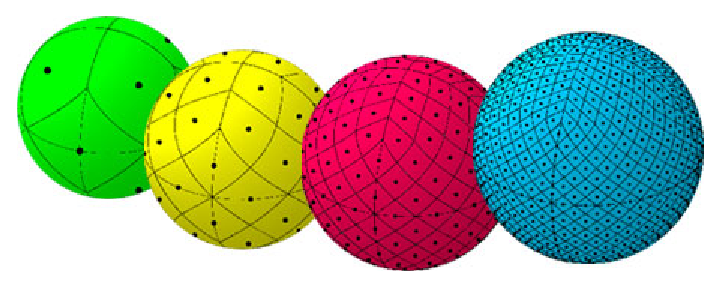
\includegraphics[width=1\linewidth]{healpixnasa}}
\caption{Разбиение HEALPix.}
\label{img:healpixnasa}
\end{figure}

\begin{figure}[h!]
\center{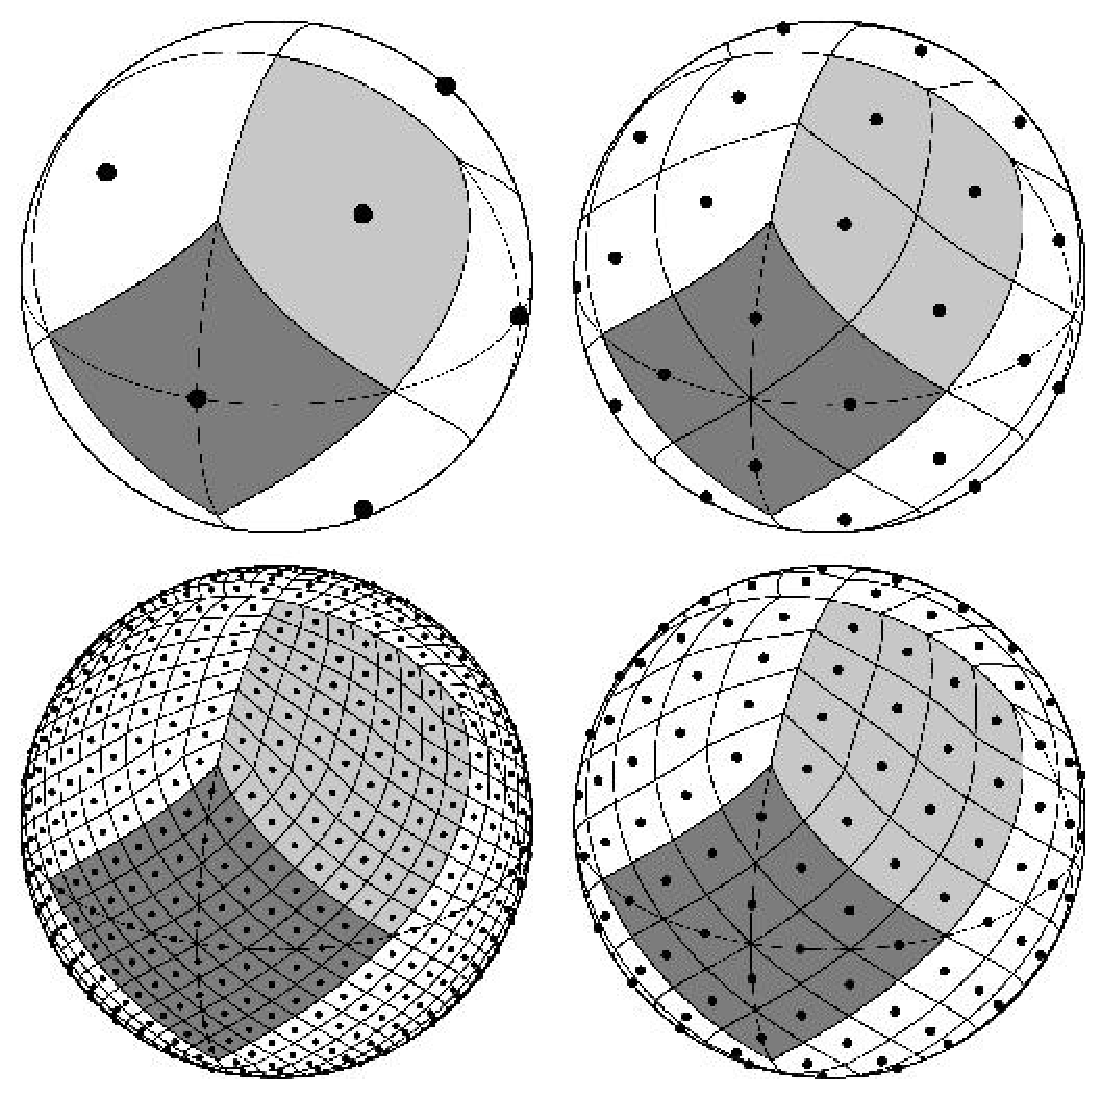
\includegraphics[width=0.5\linewidth]{healpix}}
\caption{Деление сферы на равные по пложади сигменты.}
\label{img:healpix}
\end{figure}

Другим свойством сетки HEALPix является то, что пиксельные центы, представленные черными точками, встречаются на дискретном/конечном(?) числе колец постоянной широты, количество колец зависит от разрешения сетки HEALPix. Для примера, у зеленогой, желтой, красной и синей сферы их 3, 7, 15, 31 кольцо с постоянной широтой соответственно(?).

Ниже приведён пример применения HEALPix с высоким разрешением -- Модель реликтового излучения (CMB) (космическое сверхвысокочастотное фоновое излучение), состоящая из 12582912 пикселей (~ 3.4 минут дуги (arcmin)).


\begin{figure}[h]
\begin{minipage}[h]{0.3\linewidth}
\center{
\includegraphics[width=1\linewidth]{exampleCMB} \\На сфере}
\end{minipage}
\hfill
\begin{minipage}[h]{0.69\linewidth}
\center{\includegraphics[width=0.85\linewidth]{planck2015_cmb_3000_cropped} \\Проекция Hammer}
\end{minipage}
\caption{Визуализация CMB на HEALPix}
\label{ris:image1}
\end{figure}


HealPix имеет два режима резбиения:
\begin{itemize}
\item NEST - позволяет работать со сферическими функциями и не только...

\item RING - позволяет определять минимальное расстояние до точек и не только...
\end{itemize}

\begin{figure}[h]
\begin{minipage}[h]{0.48\linewidth}
\center{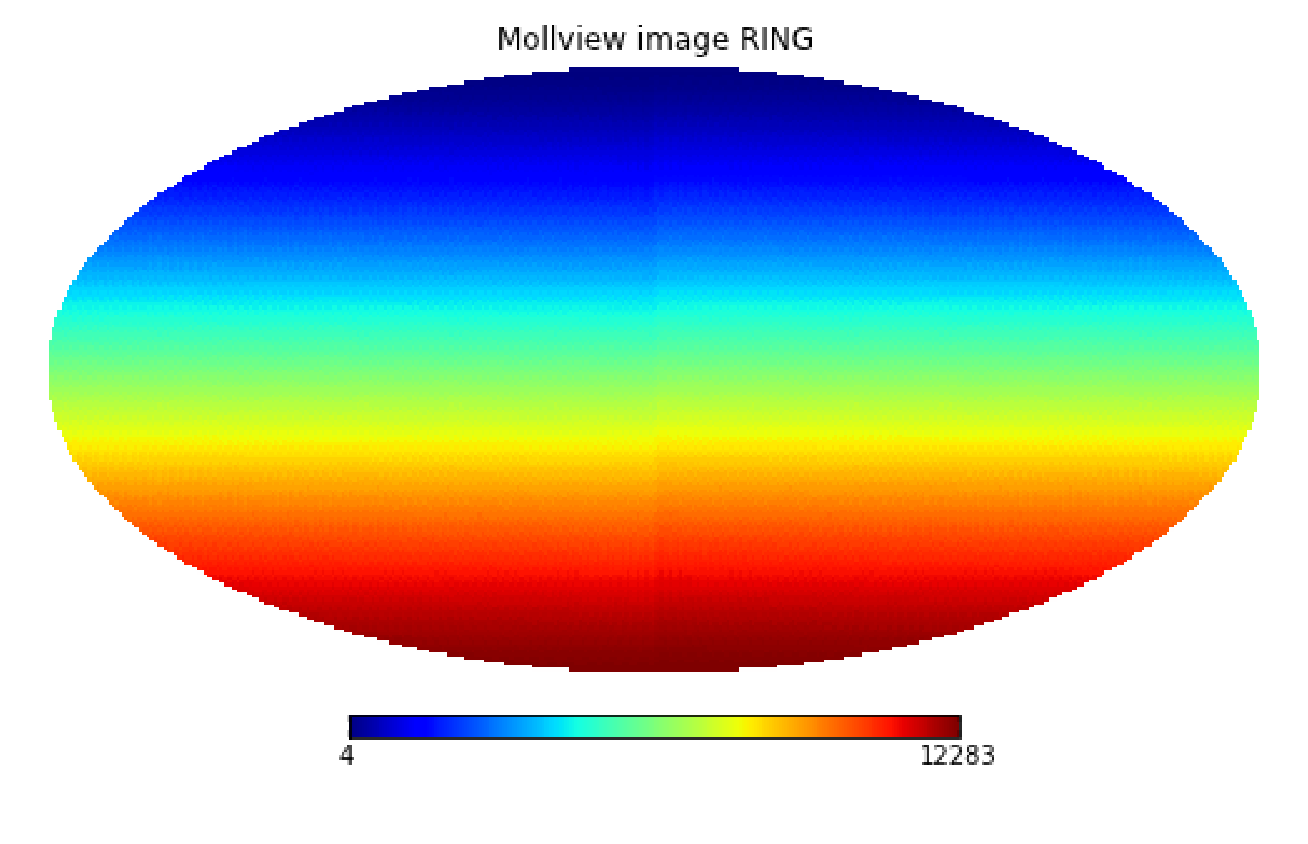
\includegraphics[width=1\linewidth]{moll_nside32_ring}}
\end{minipage}
\hfill
\begin{minipage}[h]{0.48\linewidth}
\center{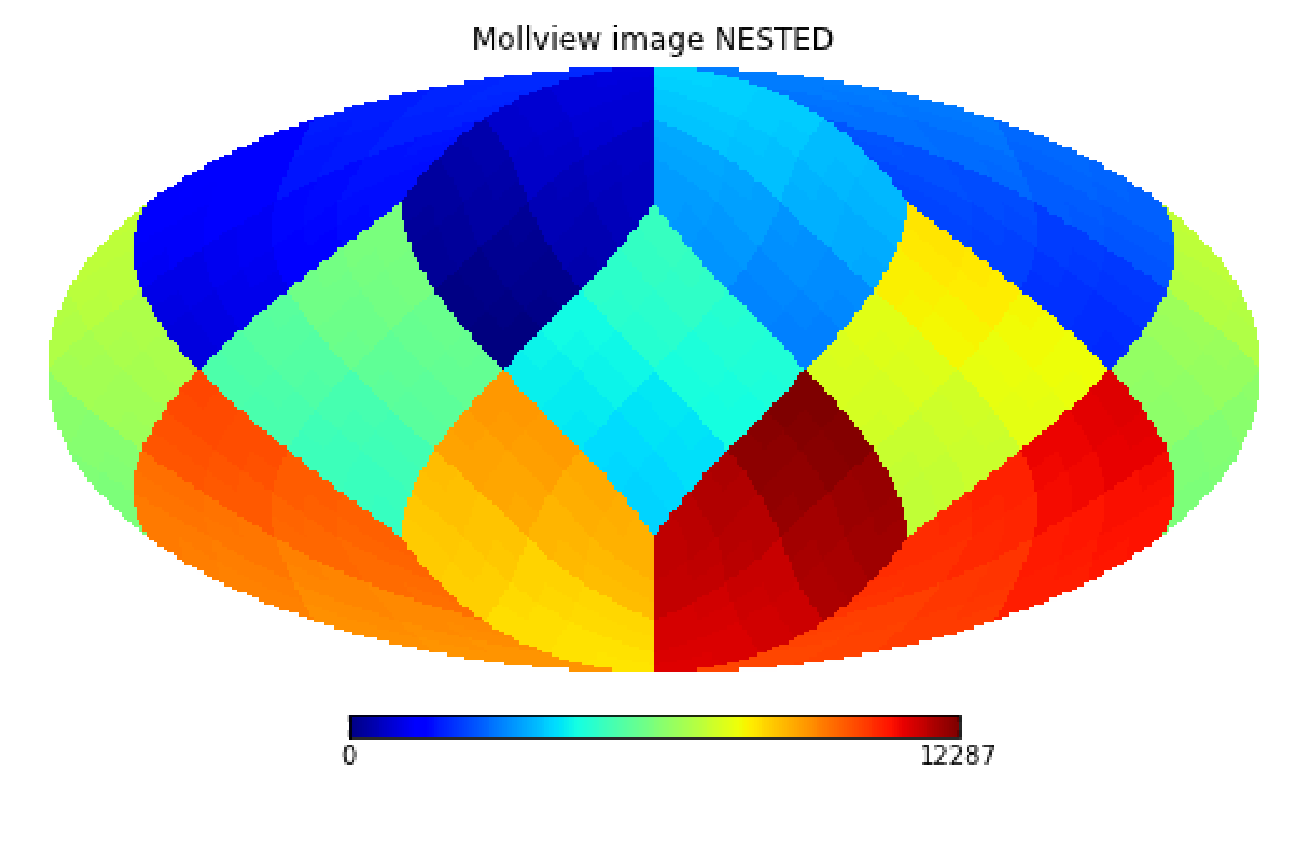
\includegraphics[width=1\linewidth]{moll_nside32_nest}}
\end{minipage}
\caption{Пример распределения  пикселей по ring and nest}
\label{ris:moll_nside32_healpix}
\end{figure}

Для нашей задачи отлично подходит NEST.

~\cite{wiki:healpix} 


\subsection{Сферические функции}\label{sub:smthsf}
Сферичекие функции -- это очень полезный инстурумент при анализе небесной сферы ~\ref{img:sf} .
~\cite{book:sf}

\begin{figure}[h!]
\center{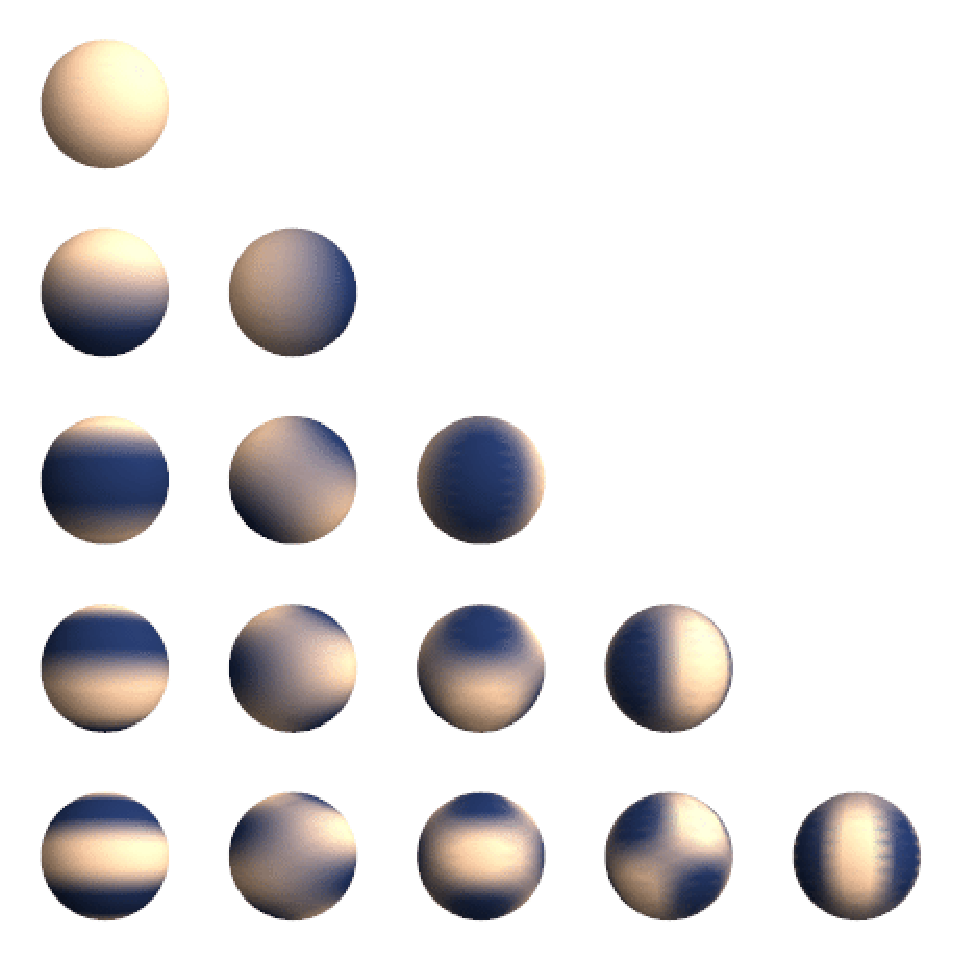
\includegraphics[width=0.5\linewidth]{Rotating_spherical_harmonics-0}}
\caption{Вещественные сферические функции $Y_{lm}$, $l=0…4$ (сверху вниз), $m=0…4$ (слева направо). Функции отрицательного порядка $Y_{l-m}$ повёрнуты вокруг оси Z на 90/m градусов относительно функций положительного порядка.}
\label{img:sf}
\end{figure}



\section{Заключение}\label{conclusion}
		ну вот и всё \cite{book:fourier} 

\newpage
\section{Список использованной литературы}\label{conclusionlit}
%\bibliographystyle{unsrt}
%\bibliography{kursach.bib}
\printbibliography[type=online,title={Online only}]
\printbibliography[type=book,title={Статьи:}]


\appendix

\section*{Приложение}
тут аппендикс или два 

\end{document}

